%
% kernbilder.tex
%
% (c) 2021 Prof Dr Andreas Müller, OST Ostschweizer Fachhochschule
%
\bgroup

\definecolor{grueneins}{rgb}{0.0,0.4,0.0}
\definecolor{gruenzwei}{rgb}{0.0,0.4,0.8}
\definecolor{orangeeins}{rgb}{1.0,0.6,0.0}
\definecolor{orangezwei}{rgb}{0.8,0.0,0.4}

\begin{frame}[t]
\frametitle{Kerne und Bilder}
\vspace{-15pt}
\begin{center}
\begin{tikzpicture}[>=latex,thick]

\uncover<2->{
\begin{scope}[xshift=-4cm,yshift=1.9cm]
\node at (0,0) {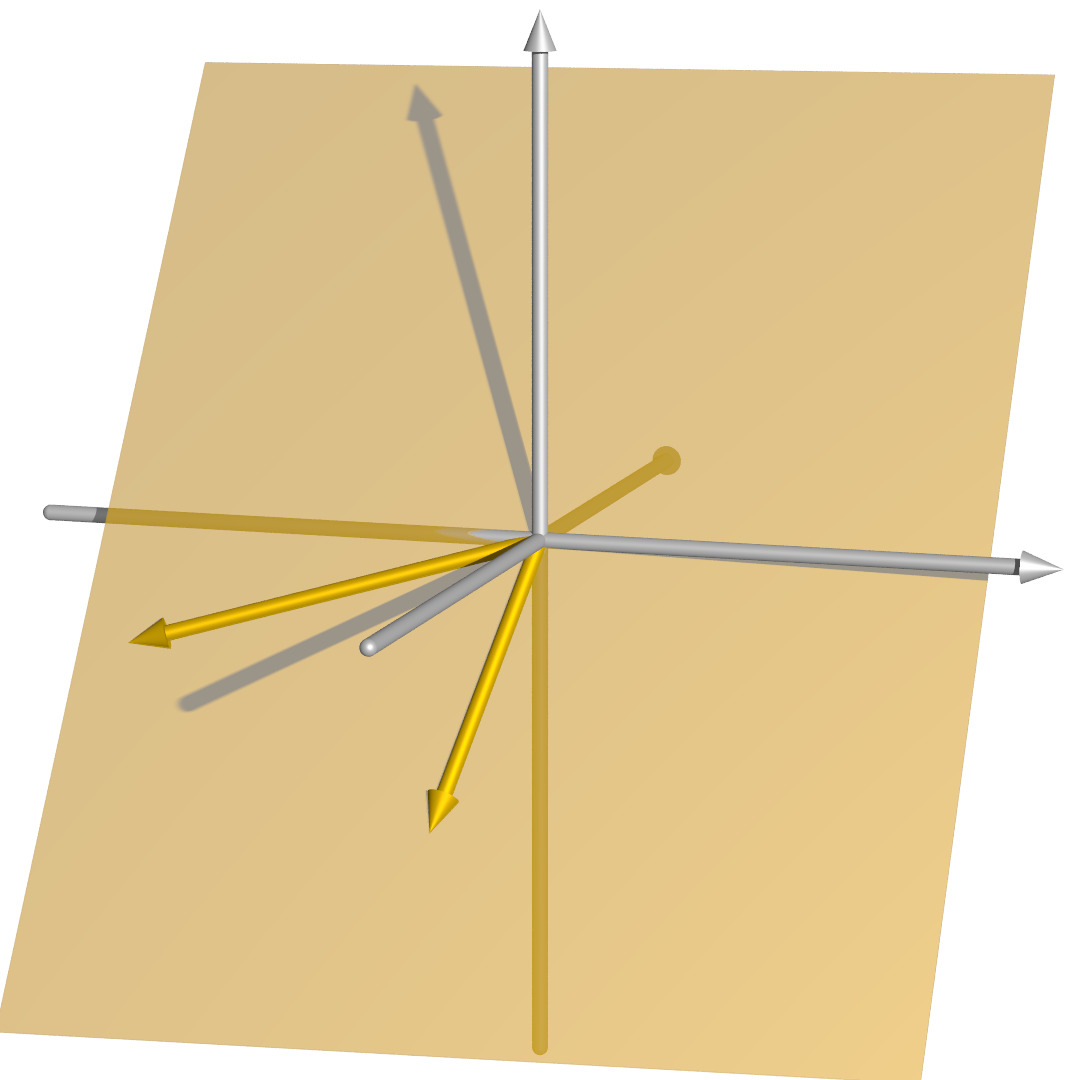
\includegraphics[width=3.6cm]{../slides/5/beispiele/bild1.jpg}};
\node[color=orangeeins] at (1.6,1.3) [right] {$\mathcal{J}^1(A)$};
\end{scope}
}

\uncover<3->{
\begin{scope}[xshift=-4cm,yshift=-1.9cm]
\node at (0,0) {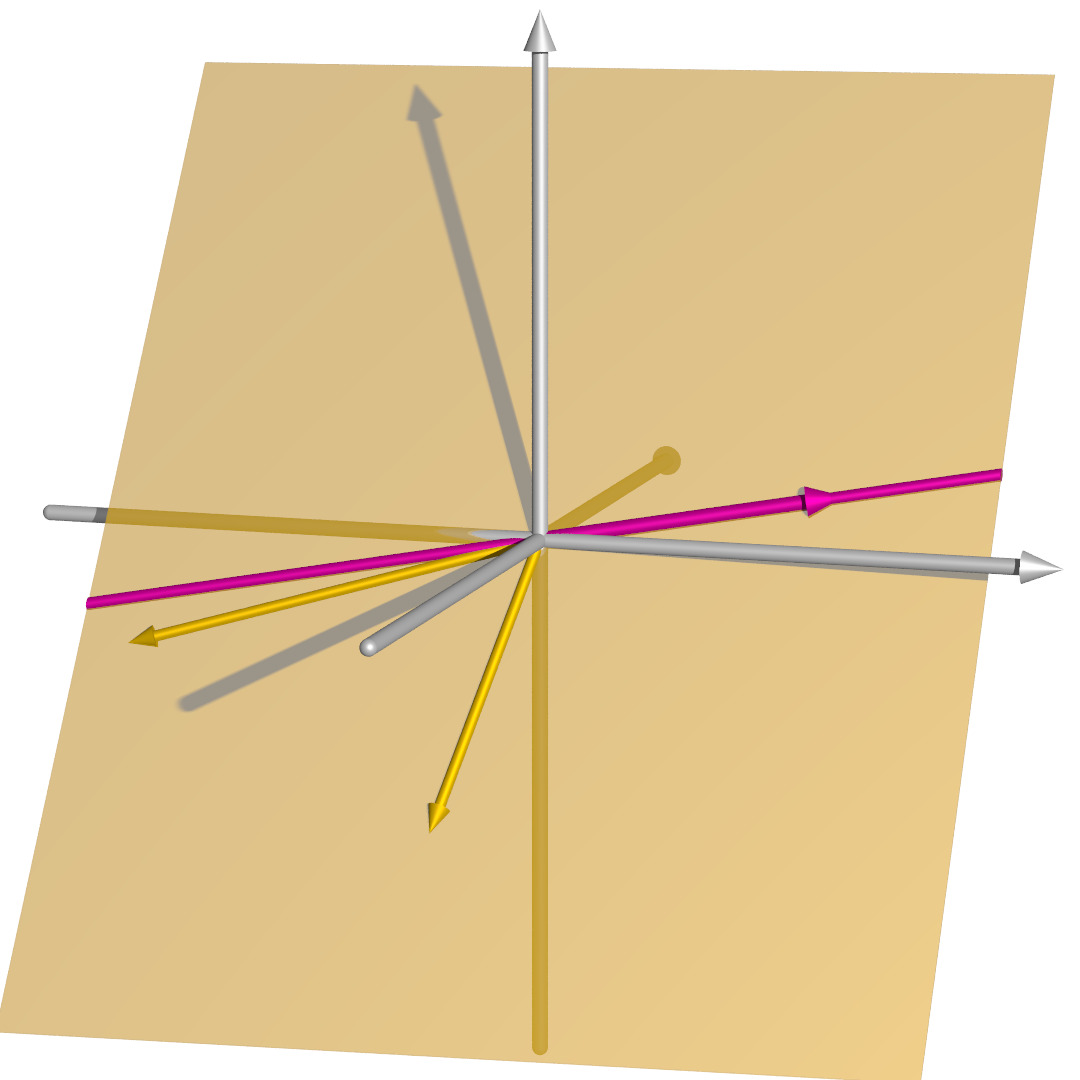
\includegraphics[width=3.6cm]{../slides/5/beispiele/bild2.jpg}};
\node[color=orangezwei] at (0.9,0.5) {$\mathcal{J}^2(A)$};
\end{scope}
}

\begin{scope}[xshift=0cm,yshift=0cm]
\uncover<1>{
\node at (0,0) {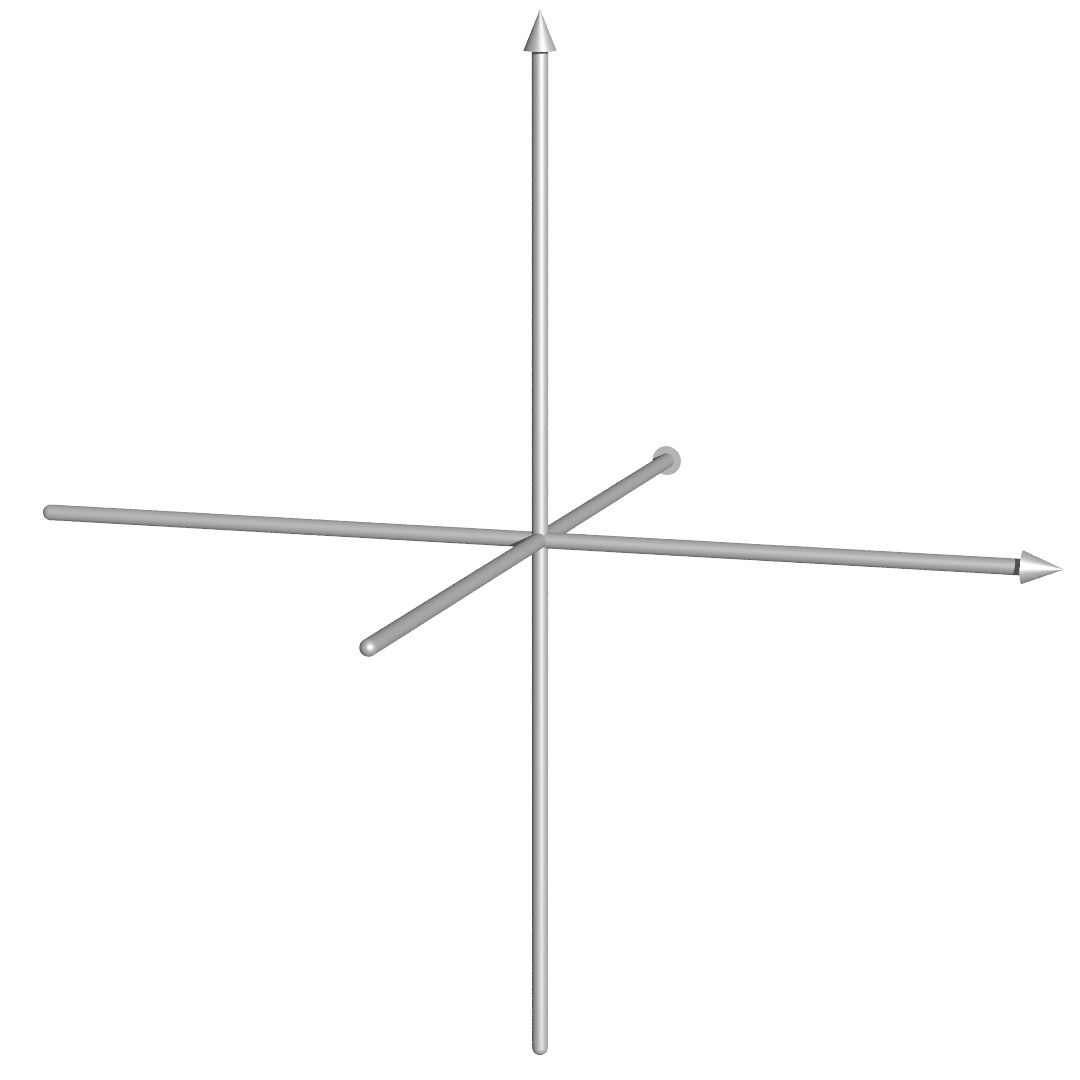
\includegraphics[width=3.6cm]{../slides/5/beispiele/leer.jpg}};
}
\uncover<2>{
\node at (0,0) {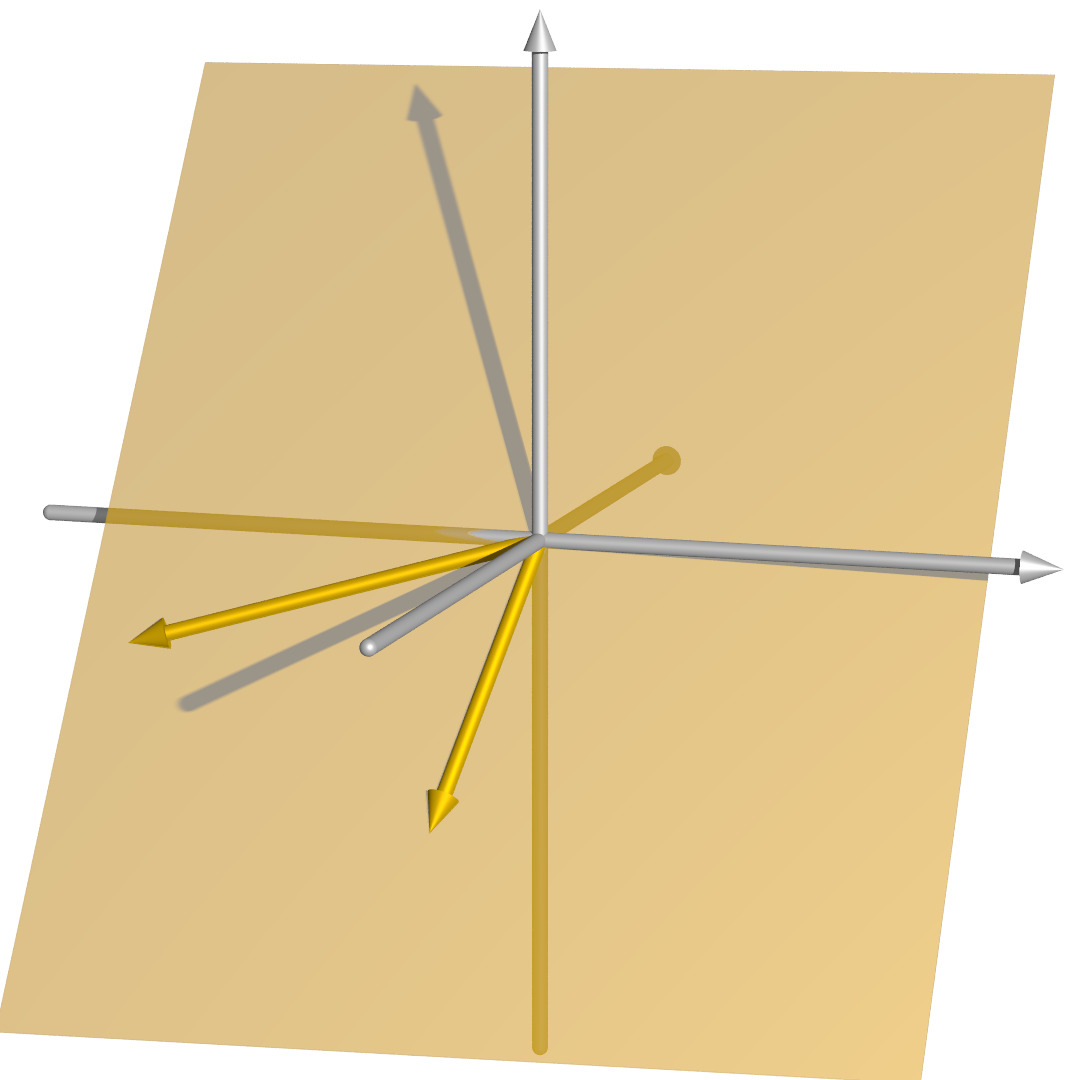
\includegraphics[width=3.6cm]{../slides/5/beispiele/bild1.jpg}};
}
\uncover<3>{
\node at (0,0) {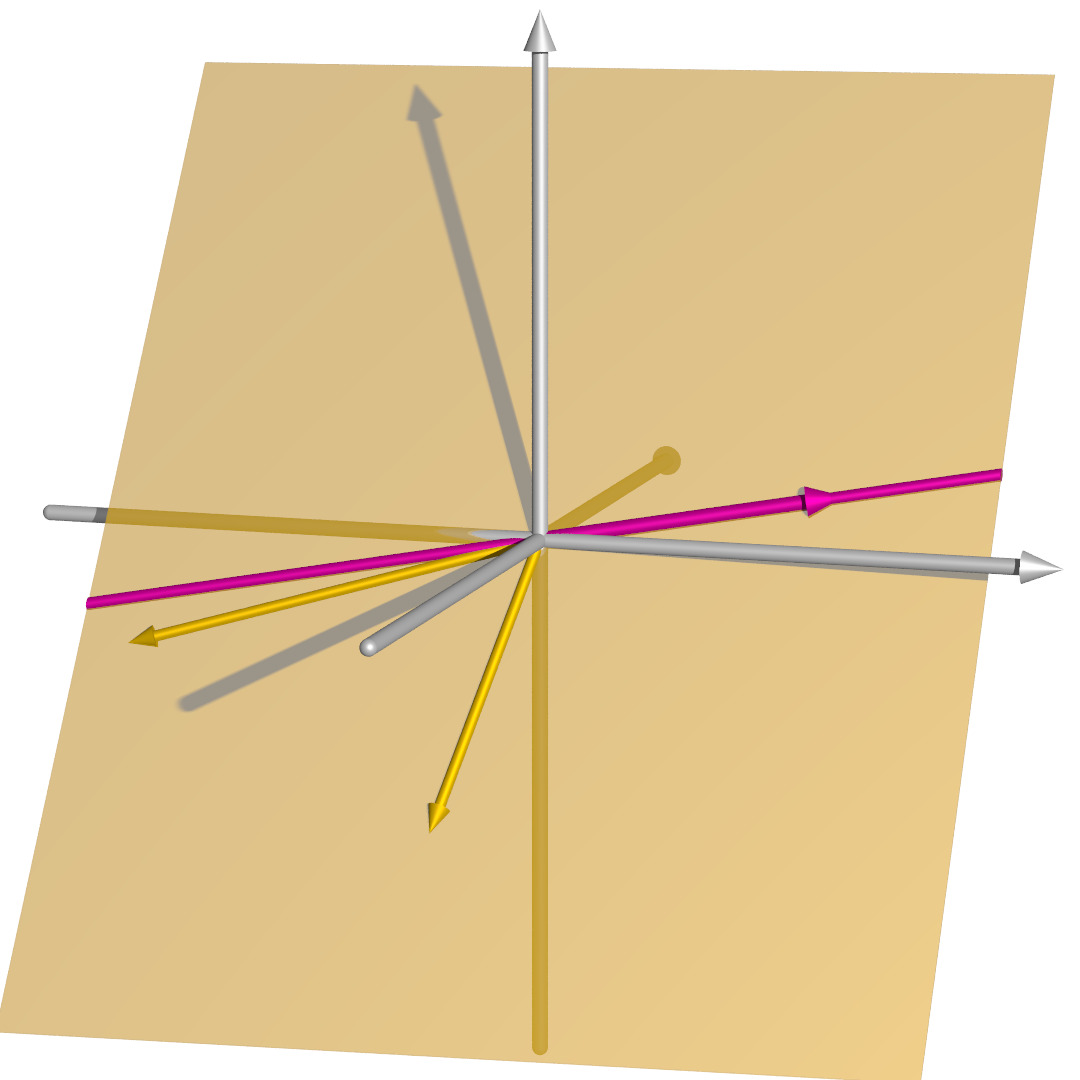
\includegraphics[width=3.6cm]{../slides/5/beispiele/bild2.jpg}};
}
\uncover<4>{
\node at (0,0) {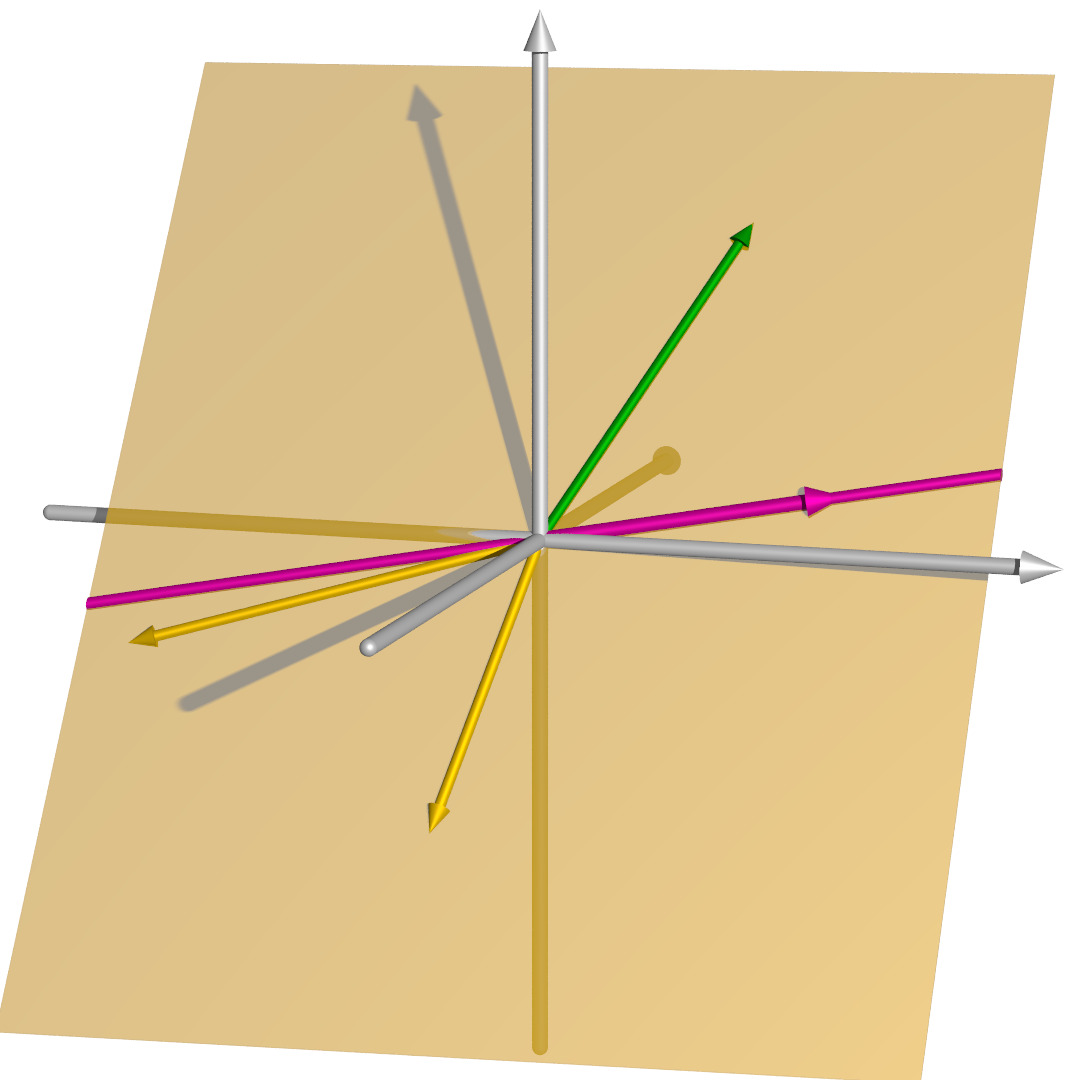
\includegraphics[width=3.6cm]{../slides/5/beispiele/drei.jpg}};
}
\uncover<5->{
\node at (0,0) {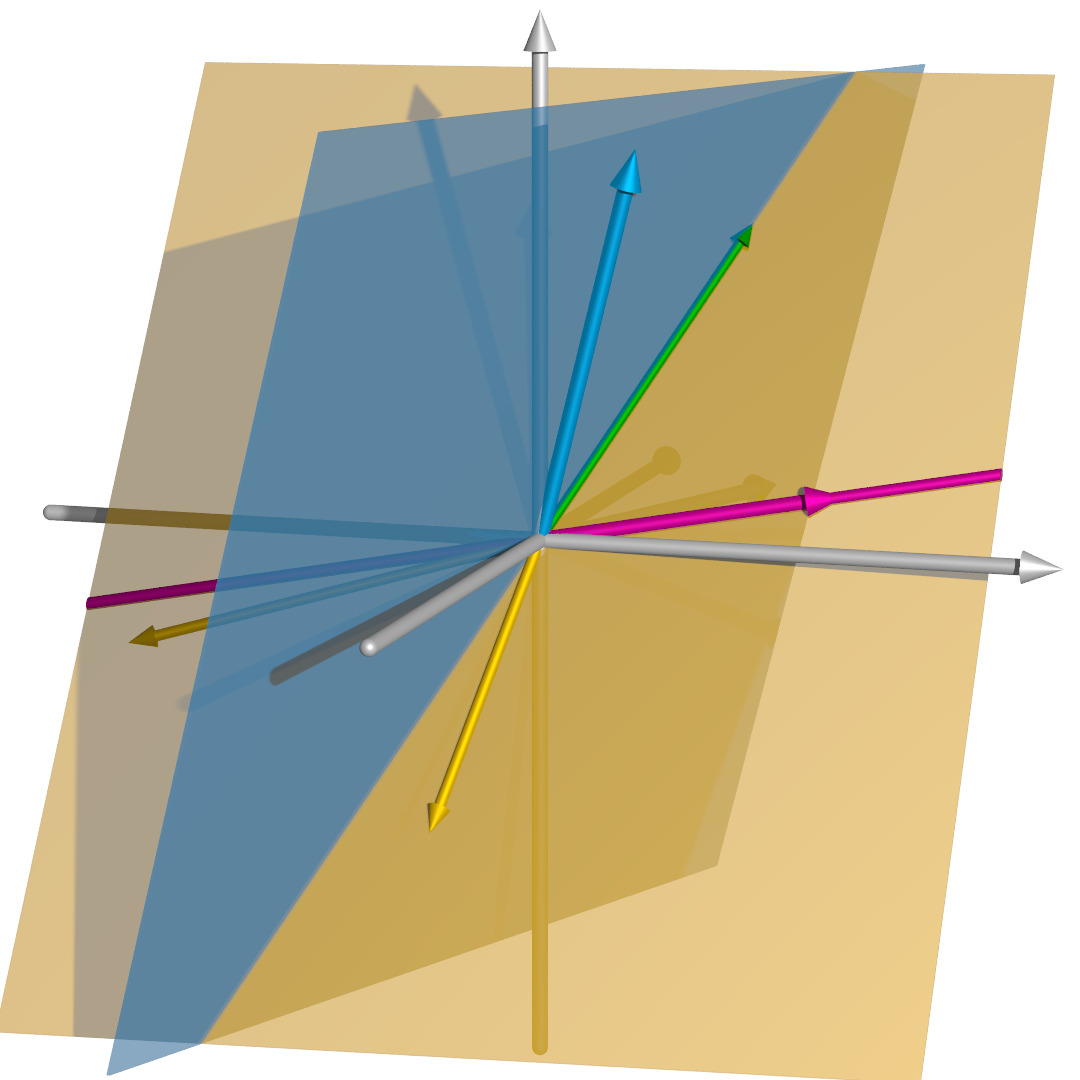
\includegraphics[width=3.6cm]{../slides/5/beispiele/kombiniert.jpg}};
}
\end{scope}

\uncover<4->{
\begin{scope}[xshift=4cm,yshift=1.9cm]
\node at (0,0) {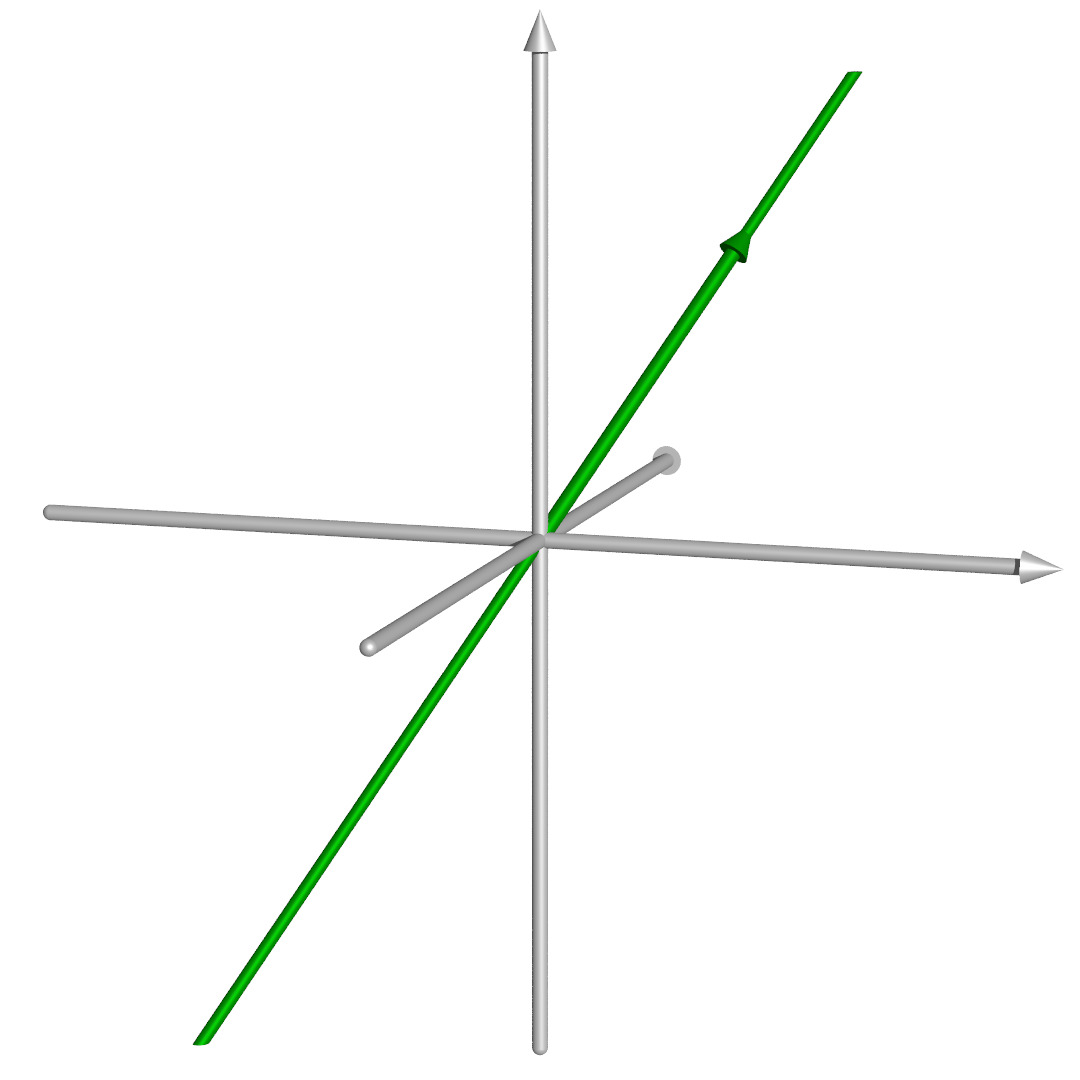
\includegraphics[width=3.6cm]{../slides/5/beispiele/kern1.jpg}};
\node[color=grueneins] at (1.0,1.3) [right] {$\mathcal{K}^1(A)$};
\end{scope}
}

\uncover<5->{
\begin{scope}[xshift=4cm,yshift=-1.9cm]
\node at (0,0) {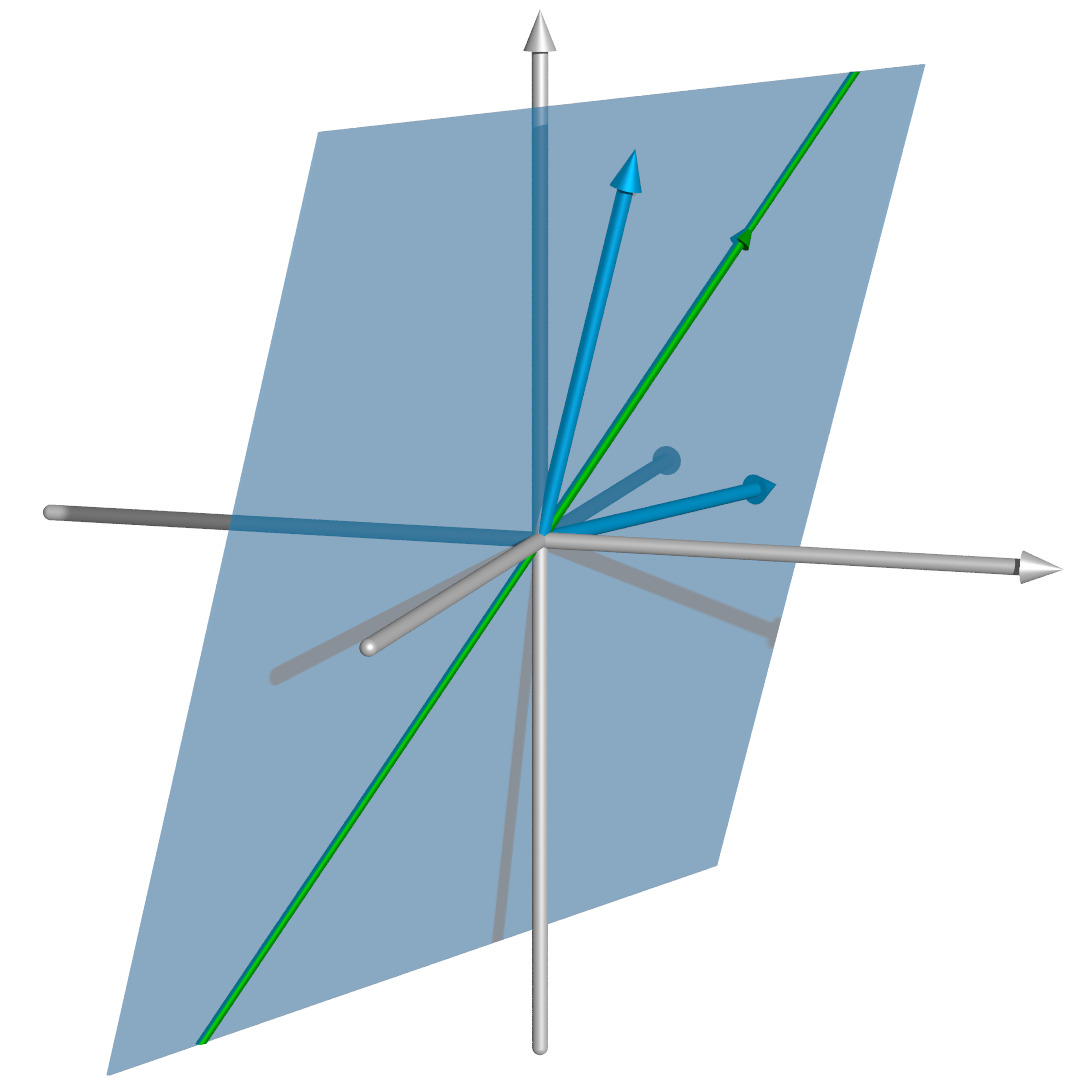
\includegraphics[width=3.6cm]{../slides/5/beispiele/kern2.jpg}};
\node[color=gruenzwei] at (0.7,-0.6) {$\mathcal{K}^2(A)$};
\end{scope}
}

\end{tikzpicture}
\end{center}
\end{frame}
\egroup
